\documentclass[a4paper,11pt,fleqn,twoside,openright]{memoir} % Brug openright hvis chapters skal starte p� h�jresider; openany, oneside
%\usepackage{fancyhdr}%mega nemt sidehoved/fod%virker ikke med memoir �benbart
%%%% PACKAGES %%%%

%\usepackage[T1]{fontenc}
%\usepackage{pgfplots}%Ting til grafer (sat ind december 2012)
%\pgfplotsset{
%  compat=newest,
%  xlabel near ticks,
%  ylabel near ticks
%} Ting til grafer (sat ind december 2012)

\usepackage[english]{babel}							% Dansk sporg, f.eks. tabel, figur og kapitel
%\usepackage{pst-plot,pst-node}
%\usepackage[pdf]{pstricks} % G�r det muligt at tegne vektor grafik.
%\usepackage{auto-pst-pdf,pstricks-add}
% �� Overs�ttelse og tegns�tning �� %
%\usepackage[ansinew]{inputenc}					% G�r det muligt at bruge �, � og � i sine .tex-filer

%\usepackage[T1]{fontenc}								% Hj�lper med orddeling ved �, � og �. S�tter fontene til at v�re ps-fonte, i stedet for bmp					

% �� FONTS �� % LaTeX er fanme ringe til skrifttyper!
%\usepackage{txfonts}									% konflikter med et eller andet.. giver i hvert fald fejl
\usepackage{mathptmx}								% times (den vi normalt bruger - bare ingen fed mat skrift)
%\usepackage{fourier}									% s�dan lidt middle ground mellem times og pazo (har heller ikke mathbf)
%\usepackage{mathpazo}								% Har fed tekst i matematik (minus mathbf), grim almindelig skrift
%\usepackage{mtpro2}									% f�lger ikke med som standard, men hvis nogen kan installere det skal de da v�re velkomne

\usepackage{latexsym}										% LaTeX symboler
\usepackage{xcolor,ragged2e,fix-cm}			% Justering af elementer
\usepackage{pdfpages}										% G�r det muligt at inkludere pdf-dokumenter med kommandoen \includepdf[pages={x-y}]{fil.pdf}	
\pretolerance=2500 											% G�r det muligt at justre afstanden med ord (h�jt tal, mindre orddeling og mere space mellem ord)
\usepackage{ulem}                       % Gennemstregning af ord med koden \sout{}
\usepackage{fixltx2e}										% Retter forskellige bugs i LaTeX-kernen
\usepackage[shortlabels]{enumitem}			% Muligg�r enkelt konfiguration af lister
\usepackage{alltt}											% Bruges af highlighting (matlab kode)
%\usepackage{Lastpage}

%Matlab kode hightlighting
 \definecolor{string}{rgb}{0.7,0.0,0.0}
    \definecolor{comment}{rgb}{0.13,0.54,0.13}
    \definecolor{keyword}{rgb}{0.0,0.0,1.0}
											
%Include cpp coding in text
\usepackage{listings}
\usepackage{color}

\definecolor{dkgreen}{rgb}{0,0.6,0}
\definecolor{gray}{rgb}{0.5,0.5,0.5}
\definecolor{mauve}{rgb}{0.58,0,0.82}

\lstset{frame=tb,
  language=C++,  
  aboveskip=3mm,
  belowskip=3mm,
  showstringspaces=false,
  columns=flexible,
  basicstyle={\small\ttfamily},
  numbers=none,
  numberstyle=\tiny\color{gray},
  keywordstyle=\color{blue},
  commentstyle=\color{dkgreen},
  stringstyle=\color{mauve},
  breaklines=true,
  breakatwhitespace=true,
  tabsize=3
}											
																			
% �� Figurer og tabeller � floats  �� %
\usepackage{flafter}										% S�rger for at dine floats ikke optr�der i teksten f�r de er sat ind.
\usepackage{multirow}                		% Fletning af r�kker
\usepackage{hhline}                   	% Dobbelte horisontale linier
\usepackage{multicol}         	        % Fletning af kolonner
\usepackage{colortbl} 									% Mulig�re farver i tabeller
\usepackage{rotating}										% Muligg�r rotation af tekst i tabeller med \begin{sideways}...\end{sideways}
\usepackage{wrapfig}										% Inds�ttelse af figurer omsv�bt af tekst. \begin{wrapfigure}{Placering}{St�rrelse}
\usepackage{graphicx} 									% Pakke til jpeg/png billeder
%\pdfoptionpdfminorversion=6%							% Muligg�r inkludering af pdf dokumenter, af version 1.6 og h�jere
\usepackage{tabularx} %Muligg�r at man kan str�kke en tabel-kolonne til �nsket l�ngde
\newsubfloat{figure}
\usepackage{epstopdf}

% �� Matematiske formler og maskinkode ��
\usepackage{amsmath, amssymb} 	% Bedre matematik og ekstra fonte 
\usepackage{textcomp}                 	% Adgang til tekstsymboler
\usepackage{mathtools}									% Udvidelse af amsmath-pakken. 
\usepackage{eso-pic}										% Tilf�j billedekommandoer p� hver side
\usepackage{lipsum}											% Dummy text \lipsum[..]



% �� Referencer, bibtex og url'er �� %
\usepackage{url}												% Til at s�tte urler op med. Virker sammen med hyperref
\usepackage[english]{varioref}						% Giver flere bedre mulighed for at lave krydshenvisninger
%\usepackage{natbib}											% Litteraturliste med forfatter-�r og nummerede referencer
%\usepackage{cite} 												% G�r det muligt at nummere kilder
\usepackage{xr}													% Referencer til eksternt dokument med \externaldocument{<NAVN>}
\usepackage{nomencl}										% Pakke til at danne nomenklaturliste
\makenomenclature												% Nomenklaturliste


% �� Floats �� %
\let\newfloat\relax 										% Memoir har allerede defineret denne, men det g�r float pakken ogs�
\usepackage{float}

\usepackage[footnote,draft,english,silent,nomargin]{fixme}		% Inds�t rettelser og lignende med \fixme{...} Med final i stedet for draft, udl�ses en error 																															for hver fixme, der ikke er slettet, n�r rapporten bygges.

%%%% CUSTOM SETTINGS %%%%

% �� Marginer �� %
\setlrmarginsandblock{3.5cm}{2.5cm}{*}	% \setlrmarginsandblock{Indbinding}{Kant}{Ratio}
\setulmarginsandblock{2.5cm}{3.0cm}{*}	% \setulmarginsandblock{Top}{Bund}{Ratio}
\checkandfixthelayout 									% Laver forskellige beregninger og s�tter de almindelige l�ngder op til brug ikke memoir pakker

%	�� Afsnitsformatering �� %
\setlength{\parindent}{0mm}           	% St�rrelse af indryk
\setlength{\parskip}{4mm}          			% Afstand mellem afsnit ved brug af double Enter
\linespread{1,1}												% Linie afstand

% �� Litteraturlisten �� %
%\bibpunct[,]{[}{]}{;}{a}{,}{,} 					% Definerer de 6 parametre ved Harvard henvisning (bl.a. parantestype og seperatortegn)
%\bibliographystyle{bibtex/harvard}			% Udseende af litteraturlisten. Ligner dk-apali - mvh Klein

% �� Indholdsfortegnelse �� %
\setsecnumdepth{subsection}		 					% Dybden af nummerede overkrifter (part/chapter/section/subsection)
\maxsecnumdepth{subsection}							% �ndring af dokumentklassens gr�nse for nummereringsdybde
\settocdepth{subsection} 								% Dybden af indholdsfortegnelsen

% �� Lister �� %
\setlist{
  topsep=-1ex,														% Vertikal afstand mellem tekst og listen
  itemsep=-1ex,													% Vertikal afstand mellem items
  partopsep=-0ex,
  parsep=1ex
} 

% �� Visuelle referencer �� %
\usepackage[colorlinks]{hyperref}			 	% Giver mulighed for at ens referencer bliver til klikbare hyperlinks. .. [colorlinks]{..}
\hypersetup{pdfborder = 0}							% Fjerner ramme omkring links i fx indholsfotegnelsen og ved kildehenvisninger ��
\hypersetup{														%	Ops�tning af farvede hyperlinks
    colorlinks = false,
    linkcolor = black,
    anchorcolor = black,
    citecolor = black
}

\definecolor{gray}{gray}{0.80}					% Definerer farven gr�

% �� Ops�tning af figur- og tabeltekst �� %
 	\captionnamefont{
 		\small\bfseries\itshape}						% Ops�tning af tekstdelen ("Figur" eller "Tabel")
  \captiontitlefont{\small}							% Ops�tning af nummerering
  \captiondelim{. }											% Seperator mellem nummerering og figurtekst
  \hangcaption													%	Venstrejusterer flere-liniers figurtekst under hinanden
  \captionwidth{\linewidth}							% Bredden af figurteksten
	\setlength{\belowcaptionskip}{-15pt}		% Afstand under figurteksten
		
% �� Navngivning �� %
\addto\captionsenglish{
	\renewcommand\appendixname{Appendix}
	\renewcommand\contentsname{Table of Contents}	
	\renewcommand\appendixpagename{Appendix}
	\renewcommand\cftchaptername{\chaptername~}				% Skriver "Kapitel" foran kapitlerne i indholdsfortegnelsen
	\renewcommand\cftappendixname{\appendixname~}			% Skriver "Bilag" foran bilagene i indholdsfortegnelsen
	\renewcommand\appendixtocname{Appendix}
}

% �� Kapiteludssende �� %


\definecolor{numbercolor}{gray}{0.7}			% Definerer en farve til brug til kapiteludseende
\newif\ifchapternonum

\makechapterstyle{jenor}{									% Definerer kapiteludseende -->
  \renewcommand\printchaptername{}
  \renewcommand\printchapternum{}
  \renewcommand\printchapternonum{\chapternonumtrue}
  \renewcommand\chaptitlefont{\fontfamily{pbk}\fontseries{db}\fontshape{n}\fontsize{25}{35}\selectfont\raggedleft}
  \renewcommand\chapnumfont{\fontfamily{pbk}\fontseries{m}\fontshape{n}\fontsize{1in}{0in}\selectfont\color{numbercolor}}
  \renewcommand\printchaptertitle[1]{%
    \noindent
    \ifchapternonum
    \begin{tabularx}{\textwidth}{X}
    {\let\\\newline\chaptitlefont ##1\par} 
    \end{tabularx}
    \par\vskip-2.5mm\hrule
    \else
    \begin{tabularx}{\textwidth}{Xl}
    {\parbox[b]{\linewidth}{\chaptitlefont ##1}} & \raisebox{-15pt}{\chapnumfont \thechapter}
    \end{tabularx}
    \par\vskip2mm\hrule
    \fi
  }
}																						% <--

%BLUEBOX KAPITEL
\newsavebox{\ChpNumBox}
\definecolor{ChapBlue}{rgb}{1,0,0} % !!
\makeatletter
\newcommand*{\thickhrulefill}{%
\leavevmode\leaders\hrule height 1\p@ \hfill \kern \z@}
\newcommand*\BuildChpNum[2]{%
\begin{tabular}[t]{@{}c@{}}
\makebox[0pt][c]{#1\strut} \\[.5ex]
\colorbox{ChapBlue}{%
\rule[-10em]{0pt}{0pt}%
\rule{1ex}{0pt}\color{black}#2\strut
\rule{1ex}{0pt}}%
\end{tabular}}
\makechapterstyle{BlueBox}{%
\renewcommand{\chapnamefont}{\large\scshape}
\renewcommand{\chapnumfont}{\Huge\bfseries} 		
\renewcommand{\chaptitlefont}{\raggedright\Huge\scshape} % \bfseries
\setlength{\beforechapskip}{10pt}	%DEFAULT:20pt
\setlength{\midchapskip}{20pt}	%DEFAULT:26pt
\setlength{\afterchapskip}{15pt}	%DEFAULT:40pt !!
\renewcommand{\printchaptername}{}
\renewcommand{\chapternamenum}{}
\renewcommand{\printchapternum}{%
\sbox{\ChpNumBox}{%
\BuildChpNum{\chapnamefont\@chapapp}%
{\chapnumfont\thechapter}}}
\renewcommand{\printchapternonum}{%
\sbox{\ChpNumBox}{%
\BuildChpNum{\chapnamefont\vphantom{\@chapapp}}%
{\chapnumfont\hphantom{\thechapter}}}}
\renewcommand{\afterchapternum}{}
\renewcommand{\printchaptertitle}[1]{%
\usebox{\ChpNumBox}\hfill
\parbox[t]{\hsize-\wd\ChpNumBox-1em}{%
\vspace{\midchapskip}%
\thickhrulefill\par
\chaptitlefont ##1\par}}%
}


% Valg af kapiteludseende - dette kan udskiftes efter �nske
%\chapterstyle{madsen}	%P1-style		
\chapterstyle{BlueBox}									

% �� Sidehoved �� %

\makepagestyle{custom}		% Definerer sidehoved og sidefod - kan modificeres efter �nske -->
\makepsmarks{custom}{																						
\def\chaptermark##1{\markboth{\itshape\thechapter. ##1}{}}		% Henter kapitlet den p�g�ldende side h�rer under med kommandoen \leftmark. \itshape g�r teksten kursiv
\def\sectionmark##1{\markright{\thesection. ##1}{}}					% Henter afsnittet den p�g�ldende side h�rer under med kommandoen \rightmark
}																														% Sidetallet skrives med kommandoen \thepage	
\makeevenhead{custom}{Computational Physics}{}{\leftmark}							% Definerer lige siders sidehoved efter modellen \makeevenhead{Navn}{Venstre}{Center}{H�jre}
\makeoddhead{custom}{\rightmark}{}{University of Oslo}			% Definerer ulige siders sidehoved efter modellen \makeoddhead{Navn}{Venstre}{Center}{H�jre}
\makeevenfoot{custom}{\thepage}{}{}													% Definerer lige siders sidefod efter modellen \makeevenfoot{Navn}{Venstre}{Center}{H�jre}
\makeoddfoot{custom}{}{}{\thepage}														% Definerer ulige siders sidefod efter modellen \makeoddfoot{Navn}{Venstre}{Center}{H�jre}		
\makeheadrule{custom}{\textwidth}{0.5pt}											% Tilf�jer en streg under sidehovedets indhold
\makefootrule{custom}{\textwidth}{0.5pt}{1mm}								% Tilf�jer en streg under sidefodens indhold

\copypagestyle{nychapter}{custom}														% F�lgende linier s�rger for, at sidefoden bibeholdes p� kapitlets f�rste side
\makeoddhead{nychapter}{}{}{}
\makeevenhead{nychapter}{}{}{}
\makeheadrule{nychapter}{\textwidth}{0pt}
\aliaspagestyle{chapter}{nychapter}													% <--

\pagestyle{custom} %normalt plain% Valg af sidehoved og sidefod
\usepackage[left=2.4cm, right=2.4cm, top=3cm, bottom=3cm]{geometry}	%Overrider tidliger marginer - men det er lidt mere simpelt.

%%%% CUSTOM COMMANDS %%%%
%referencer
\newcommand{\figref}[1]{Fig.~\ref{#1}}
\newcommand{\tabref}[1]{Tab.~\ref{#1}}	
\newcommand{\matref}[1]{Eq.~\eqref{#1}}
\newcommand{\chapref}[1]{Chap.~\ref{#1}}
\newcommand{\secref}[1]{Sec.~\ref{#1}}
\newcommand{\subsecref}[1]{Subsec.~\ref{#1}}
\newcommand{\appref}[1]{App.~\ref{#1}}
\newcommand{\citer}[1]{\citep[Se][]{#1}}
\newcommand{\citerk}[2][]{\citep[Se][kap.~#1]{#2}}
\newcommand{\citers}[2][]{\citep[Se][s.~#1]{#2}}


% �� Billede hack �� %
\newcommand{\figur}[4]{
		\begin{figure}[H] \centering
			\includegraphics[width=#1\textwidth]{billeder/#2}
			\caption{#3}\label{#4}
		\end{figure} 
		}
		
% �� Specielle tegn �� %
\newcommand{\grader}{\ensuremath{^{\circ}\text{C}}}
\newcommand{\gr}{\ensuremath{^{\circ}}}
\newcommand{\g}{\cdot}


% �� Promille-hack (\promille) �� %
\newcommand{\promille}{%
  \relax\ifmmode\promillezeichen
        \else\leavevmode\(\mathsurround=0pt\promillezeichen\)\fi}
\newcommand{\promillezeichen}{%
  \kern-.05em%
  \raise.5ex\hbox{\the\scriptfont0 0}%
  \kern-.15em/\kern-.15em%
  \lower.25ex\hbox{\the\scriptfont0 00}}

\newcommand{\HRule}{\rule{\linewidth}{0.5mm}}

% �� CUSTOM MATEMATIK/FYSIK-TING ��
\renewcommand{\v}[1]{\ensuremath{\mbox{\textbf{#1}}}} % for vectors
\newcommand{\gv}[1]{\ensuremath{\mbox{\boldmath$ \vec{#1}  $}}} 
% for vectors of Greek letters
\newcommand{\uv}[1]{\ensuremath{\mbox{\boldmath$ \hat{#1}  $}}}  % for unit vector
\newcommand{\abs}[1]{\left| #1 \right|} % for absolute value
\newcommand{\avg}[1]{\left< #1 \right>} % for average
\let\underdot=\d % rename builtin command \d{} to \underdot{}
\renewcommand{\d}[2]{\frac{d #1}{d #2}} % for derivatives
\newcommand{\dd}[2]{\frac{d^2 #1}{d #2^2}} % for double derivatives
\newcommand{\pd}[2]{\frac{\partial #1}{\partial #2}} 
% for partial derivatives
\newcommand{\pdd}[2]{\frac{\partial^2 #1}{\partial #2^2}} 
% for double partial derivatives
\newcommand{\pdc}[3]{\left( \frac{\partial #1}{\partial #2}
 \right)_{#3}} % for thermodynamic partial derivatives
\newcommand{\ket}[1]{\left| #1 \right>} % for Dirac bras
\newcommand{\bra}[1]{\left< #1 \right|} % for Dirac kets
\newcommand{\braket}[2]{\left< #1 \vphantom{#2} \right|
 \left. #2 \vphantom{#1} \right>} % for Dirac brackets
\newcommand{\matrixel}[3]{\left< #1 \vphantom{#2#3} \right|
 #2 \left| #3 \vphantom{#1#2} \right>} % for Dirac matrix elements
\newcommand{\grad}[1]{\gv{\nabla} #1} % for gradient
\let\divsymb=\div % rename builtin command \div to \divsymb
\renewcommand{\div}[1]{\gv{\nabla} \cdot #1} % for divergence
\newcommand{\curl}[1]{\gv{\nabla} \times #1} % for curl
\let\baraccent=\= % rename builtin command \= to \baraccent
\renewcommand{\=}[1]{\stackrel{#1}{=}} % for putting numbers above =
\renewcommand\Re{\operatorname{Re}}
\renewcommand\Im{\operatorname{Im}}
\newcommand{\comp}[1]{\widetilde{#1}}
\newcommand{\unit}[1]{\ensuremath{\, \mathrm{#1}}}

\newcommand{\eqvref}[1]{(\ref{#1}) p� side \pageref{#1}}

\newcommand{\forsog}[1]{\underline{#1}}

\newcommand{\superscript}[1]{\ensuremath{^{\textrm{#1}}}}
\newcommand{\subscript}[1]{\ensuremath{_{\textrm{#1}}}}


%%%% ORDDELING %%%%

\hyphenation{egen-skab-er egen-skab hvad hvem hvor Halv-le-der-ud-snit-tet}

% Makro til fxnotes
\newcommand{\AVP}[1]{\fxnote{\textbf{AVP}: #1}}
\newcommand{\BM}[1]{\fxnote{\textbf{BM}: #1}}
\newcommand{\flops}[1]{flops}
\raggedbottom
\begin{document}

\frontmatter	% Romertal på de første sider
\thispagestyle{empty}

\begin{center}


% Upper part of the page

\textsc{\LARGE University of Oslo}\\[0.5cm]

\textsc{\Large Computational Physics}\\[2cm]
 

% Title
\HRule \\[0.4cm]
 \LARGE \textbf{Project 5}  \\[0.2cm]
\HRule \\[2.5cm]

\vspace{2cm}

\includegraphics[width=0.8\textwidth]{Figures/UiO_Seal_A_ENG.png}\\  %Forsidebillede

\vfill 
 
% Forfattere og vejleder
\begin{tabularx}{\textwidth}{l X r}
\hline
& & \large \emph{Authors:}\\
& & \large Birgitte Madsen, 66\\
& & \large Magnus Isaksen, 14 \\
& & \large Soumya Chalakkal, 51 \\
\hline

\end{tabularx}




\vfill

% Bottom of the page
{\large Autumn 2015}

\end{center}
\cleardoublepage


\cleardoublepage		
% Dette er LaTeX-versionen af titelbladet for tek-nat-basis-rapporter 2004 efterår
% Filen kræver:
% Universitetets logo:  aau-logo.png (for LaTeX) eller aau-logo.ps (for LaTeX)
% Synopsis: En fil ved navn synopsis.tex

% Udarbejdet af: Hans HŸttel (hans@cs.auc.dk) 21. maj 2003
% Rettet af Morten Christophersen (mortench@tnb.aau.dk) 30. nov 2004(ændret til nyt design 2004 efterår)

%\documentclass[11pt]{article}
%\ifx\pdfoutput\undefined 
%\usepackage[dvips]{graphicx}
%\else
%\usepackage[pdftex]{graphicx} 
%\usepackage{type1cm} \fi
%    \usepackage[ansinew]{inputenc}
%    \usepackage{a4}

%\begin{document} 
\phantomsection
\pdfbookmark[0]{Titelblad}{titelblad}
\thispagestyle{empty}
%\begin{titlepage}
\begin{nopagebreak}
{\samepage 
\begin{tabular}{r}
\parbox{\textwidth}{  \raisebox{1mm}{
\includegraphics[height=1.5cm]{Figures/UiO_Seal_A_ENG.png}}
\hfill \parbox{5.5cm}{\begin{tabular}{r} %4.90
{\small \textbf{Department of Physics}}\\
{\small  \textbf{University of Oslo}} \\
{\small  Sem S\ae lands vei 24} \\
{\small  0371 Oslo, Norway} \\
{\small +47 22 85 64 28} \\
%{\small Fax 99 40 92 35} \\
{\small http://www.mn.uio.no/fysikk/english/}
\end{tabular}}}

\end{tabular}

\vspace{2.5cm}
\begin{tabular}{cc}
\parbox{20cm}{
\begin{description}
\item { \textbf{Course:}}

	Computational Physics\\
	\hspace{4cm}
	\vspace{0.7cm}
\item { \textbf{Project number:}}

	5 \\
	\hspace{4cm}
	\vspace{0.7cm}

\item {\textbf{Link to GitHub folder:} }

	\url{https://?????}  \\ 
	\hspace{4cm}
	\vspace{0.7cm}

\item { \textbf{Hand-in deadline:}}

   Friday, December 11, 2015\\
  \hspace{4cm}
  \vspace{0.7cm}
  
\item { \textbf{Project Members:}}

Birgitte Madsen, 66 \\
Magnus Isaksen, 14 \\
Soumya Chalakkal, 51 \\
  \hspace{2cm}
  \vspace{0.7cm}

\end{description}

\vspace{0.25cm}
\begin{description}
\item { \textbf{Copies:} 1}
\item { \textbf{Page count:} \pageref{LastPage}  } 
\item { \textbf{Appendices:} 0} 
\item { \textbf{Completed:} ????, 2015 } 
\end{description}
\vfill } &
%\parbox{7cm}{
%  \vspace{.15cm}
%  \hfill 
%  \begin{tabular}{l}
%  {\textbf{Synopsis:}}\bigskip \\
%  \fbox{
%    \parbox{6.5cm}{\bigskip
%     {\vfill{\small \input{Chapters/Formalia/synopsis.tex}
%     \bigskip}}
%     }}
%   \end{tabular}}
\end{tabular}}
\\ \\ \\ 

\noindent{\footnotesize{\textit{The content of the report is freely available, but publication (with source) may only be made with the agreement of the authors.}}}
\end{nopagebreak}
%\end{titlepage}
%\end{document}

\cleardoublepage
\chapter*{Abstract}

In this project an open cluster is simulated using two different algorithms, the fourth order Runge-Kutta and the Velocity Verlet. During the project the fourth order Runge-Kutta is chosen as the main algorithm, as it gives more stable results for a many body system. The evolution of the cluster is studied looking at the energies, the distribution of particles and positions as time progresses. Studying the energies it was found that the system lost energy as particles were ejected from the cluster. When the system reached an approximately equilibrium state after a period of $3\tau_{crunch}$, it was consistent with the virial theorem.

\cleardoublepage	
%\chapter*{Preface}
This project is written by 6th semester physics group 4.207a at the Department of Physics and
Nanotechnology at Aalborg University, Denmark, in the Spring semester, 2014, as a 10 ECTS-point bachelor project.

\subsection*{Reading Guide}
Succeeding chapters support each other, and it is therefore recommended to read the report chronologically.
When referring to equations or the like in the text, \textit{equation} will be shortened Eq., \textit{table} will be shortened Tab., and so forth.
In \appref{app:ListOfSymbols} a list of frequently used symbols and constants are given.
The external references used in this work appear in numbered order in brackets in the text and are listed in the bibliography at the end of the report in order of succession.

\subsection*{Signatures}
The group member's signatures below express that the entire group is accountable for all aspects of the project and all chapters of the report. 

\vspace{4cm}

\begin{table}[H]
	\centering
		\begin{tabular}{c c}
			\underline{\phantom{JAERJAERJAERJAERJAERJAERJAER}}	 	&	\underline{\phantom{JAERJAERJAERJAERJAERJAERJAER}} 
			\\
			Andreas V. Pedersen								& 	Birgitte Madsen	
			\\									
		\end{tabular}
\end{table}
%\cleardoublepage			
\tableofcontents*

\mainmatter % Side nummereringen starter ved 1 herfra

	\chapter{Introduction}

	\chapter{Method}
\label{chap:method} 
The methods introduced in this chapter, are used to study the evolution of bodies, also referred to as particles, in the solar system or in the galaxy. 
Firstly, the fourth order Runge-Kutta method and the Velocity-Verlet method are introduced for a 2-body problem in 3 dimensions, however, since the aim of this project is to investigate the time evolution of a star cluster consisting of $N$ particles, the code is extended to $N$ bodies by incorporating suitable changes. 

To generate the $N$ bodies, a function for generating the position coordinates of the N bodies as uniformly distributed particles within a sphere is introduced as discussed in sec \secref{Method:GeneratingPosMassVel}, along with a function for generating masses that are randomly distributed by a Gaussian distribution around ten solar masses with a standard deviation of one solar mass.

In the Github folder \url{https://github.com/birgimad/Project5_BM_MI_SC}, the source codes for the algorithms described in this chapter can be found. 


	\section{Newtonian two-body problem in three dimension}
\label{Newton2body3D}
The problem of solving the time-evolution of a two-body system in three dimensions can reasonably be considered in two different coordinate systems: one coordinate system with one of the bodies in rest compared to the frame of reference in which the other body is moving, and one coordinate system with both of the bodies moving relative to the frame of reference. 
Both of these reference systems are depicted in \figref{fig:2bodyproblem_coordinatesystems}. 
\begin{figure}[H]
\centering
	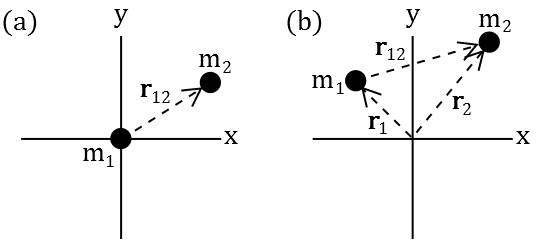
\includegraphics[width=0.6\linewidth]{Figures/2bodyproblem_coordinatesystems.png}
\caption{
Two-dimensional illustration of the three-dimensional problem of determining determining the relative distance and relative velocity between two bodies. 
In (a) body 1 with mass $m_1$ is considered stationary in position- and velocity-space, whilst body 2 with mass $m_2$ moves relative to body 1.
In (b) both body 1 and 2 moves relative to the frame of reference in position and time, yielding that the position vector between body 1 and 2 is given as $\v{r}_{12} = \v{r}_2 - \v{r}_1$.
}
\label{fig:2bodyproblem_coordinatesystems}
\end{figure}
In the codes presented in this section, solving the problem in coordinate system (a) will first be considered for simplicity. Thereafter, the codes will be extended to include the movement of body 1 relative to the coordinate system, since this will be useful when extending the codes to an N body system.  

In the problem, $\v{r}(t)$ is the three-dimensional space vector consisting of the coordinated $(x(t),y(t),z(t))$, whilst $\v{v}(t)$ is the three-dimensional velocity vector with coordinates $(v_x(t),v_y(t),v_z(t))$, both of which are dependent on time. 

In general, the considered differential equation is
\begin{align}
	\frac{dy}{dt} = f(t,y)
	\label{eq:diffEq1}
\end{align}
Which yields that
\begin{align}
	y(t) = \int f(t,y) dt
\end{align}
\fxnote{do we need to write $y_{i+1}$ eq from p. 250 in lecture notes??}
For the two bodies in a three dimensional Newtonian gravitational field this corresponds to six coupled differential equations given by the vector equations
\begin{align}
	\frac{d\v{r}}{dt} = \v{v}
	\qquad \text{and} \qquad
	\frac{d\v{v}}{dt} = - \frac{G M_1 M_2}{r^3} \v{r}
	\label{eq:diffEq2}
\end{align}
\fxnote{maybe we should divide by mass as on p. 248??}
in which $M_1$ and $M_2$ \fxnote{fix the this with $M_1$ and $M_2$} are the masses of the two bodies, respectively, whilst $r$ is the distance between the bodies.
The equations in \eqref{eq:diffEq2} are computed by the script given below in which $drdt$ corresponds to the derivative of the coordinates of the position, and $dvdt$ corresponds to the derivative of the velocity coordinates. 
\begin{lstlisting}
void Derivative(double r[3], double v[3], double (&drdt)[3], double (&dvdt)[3], double G, double mass){
    drdt[0] = v[0];
    drdt[1] = v[1];
    drdt[2] = v[2];

    double distance_squared = r[0]*r[0] + r[1]*r[1] + r[2]*r[2];
    double newtonian_force = -G*mass/pow(distance_squared,1.5);
    dvdt[0] = newtonian_force*r[0];
    dvdt[1] = newtonian_force*r[1];
    dvdt[2] = newtonian_force*r[2];
}
\end{lstlisting}

	\subsection{Velocity-Verlet method}
\label{sec:methodVV}
The basic idea of the Velocity-Verlet algorithm is to write the Taylor expansion of the position in Newton’s equation, one forward step and one backward step in time with step length $\delta t$ as
\begin{align}
	\v{r}(t_i \pm \delta t) = \v{r}(t_i) \pm \v{v} (t_i) \delta t
	+ \v{a} (t_i) \frac{\delta t ^2}{2}  \pm \frac{\delta t ^3}{6} \frac{d^3 \v{r}(t_i)}{dt^3} + \mathcal{O}(\delta t ^4 )
	\label{eq:TaylorExpVVmethod}
\end{align}
in which $\v{v}(t_i) = d\v{r}(t_i)/dt$ is the velocity, and $\v{a}(t_i) = d^2 \v{r}(t_i)/dt^2$ is the acceleration at time $t_i$.
Adding the two expressions in \matref{eq:TaylorExpVVmethod} gives
\begin{align}
	\v{r} (t_i +\delta t) = 2\v{r} (t_i) - \v{r} (t_i -\delta t)  + \v{a} (t_i ) \delta t^2 + \mathcal{O} (\delta t ^4 )
	\label{eq:TaylorExpVVmethod2}
\end{align}
which has a truncation error that goes as $\mathcal{O} (\delta t ^4 )$.
Now, using $\v{r}(t_i-\delta t) = \v{r}(t_i) - \v{v}(t_i) \delta t + \v{a} \delta t^2 /2 + \mathcal{O} (\delta t^3)$, yield that the position at time $t_i+\delta t$ can be determined as 
\begin{align}
	\v{r}(t_i+\delta t) = \v{r}(t_i) + \v{v} (t_i) \delta t + \frac{1}{2} \v{a} (t_i) \delta t^2 
	\label{eq:VVmethodNextPosition}
\end{align}
Since the velocity is not included in \matref{eq:TaylorExpVVmethod2}, it is computed through the Velocity-Verlet scheme where position, velocity and acceleration at time $t_i+\delta t$ is computed from the Taylor expansion as
\begin{align}
	\v{v} (t + \delta t) = \v{v} (t) + \frac{1}{2} ( \v{a} (t) + \v{a} (t + \delta t) ) \delta t
	\label{eq:VVmethodNextVelocity}
\end{align}
The velocity at time $t_i+\delta t$ is in the algorithm computed by first calculating 
\begin{align}
	\v{v}_{part1} (t + \delta t) = \v{v} (t) + \frac{1}{2}  \v{a} (t)  \delta t
	\label{eq:VVmethodNextVelocityPart1}
\end{align}
and then use the \textit{Derivative} function to determine $\v{a} (t + \delta t)$, which is then used to compute the remaining term of \matref{eq:VVmethodNextVelocity} as 
\begin{align}
	\v{v}_{part2} (t + \delta t) = \frac{1}{2} \v{a} (t + \delta t) \delta t
	\label{eq:VVmethodNextVelocityPart2}
\end{align}

The velocity-Verlet method uses the algortihm \textit{Derivative} described in \secref{Newton2body3D}, to generate the six differential equations, in the following while-loop that runs until reaching the final time in time steps of length $\delta t = (t_{initial} - t_{final})/(\# time steps)$.
\begin{lstlisting}
    while(time<=t_final){
    Derivative(r,v,drdt,dvdt,G,mass);
    for(int i=0; i<6 ; i++){
    r[i] = r[i]+dt*drdt[i] + 0.5 * dt * dt * dvdt[i];
    v_partly[i] = drdt[i] + 0.5 * dt * dvdt[i];
    dvdt[i] = v_partly[i];
    }
    Derivative(r,v,drdt,dvdt,G,mass);
    for(int i=0; i<n ; i++){
    v[i] = v_partly[i] + 0.5 * dt * dvdt[i];
    }
    time += dt;
    }
\end{lstlisting}	
	\subsection{Fourth Order Runge-Kutta Method}
\label{sec:methodRK4}
- Remember to write about accuracy of algorithm!!

The Runge-Kutta method is based on Taylor expansions, with the next function value after a times step $\delta t = t_i - t_{i+1}$ being computed from four more or less improved slopes of the function in the points $t_i$, $t_i + \delta t /2$ and $t_{i+1}$.
  
The first step of the RK4 method is to compute the slope $k_1$ of the function in $t_i$ by
\begin{align*}
	k_1 = \delta t f(t_i , y_i)
\end{align*}
Then the slope $k_1$ at the midpoint is computed from $k_1$ as
\begin{align*}
	k_2 = \delta t f(t_i + \delta t /2, y_i + k_1 /2 )
\end{align*}
The slope at the midpoint is then improved from $k_2$ by
\begin{align*}
	k_3 = \delta t f(t_i + \delta t /2, y_i + k_2 /2 )
\end{align*}
from which the slope $k_4$ at the next step $y_{i+1}$ is predicted to be
\begin{align*}
	k_4 = \delta t f(t_i + \delta t, y_i +k_3 )
\end{align*}
From the computed slopes $k_1$, $k_2$, $k_3$ and $k_4$, the function value at $t_i + \delta t$ is computed as
\begin{align}
 y_{i+1} = y_i + \frac{1}{6} (k_1 + 2k_2 + 2k_3 +k_4 )
 \label{eq:RK4nextxtep1}
\end{align}
When implementing this for the two-body problem in three dimensions, it boils down to a continuous call of two functions, namely the function 
\textit{Derivative} given in 
\secref{Newton2body3D} and the function 
\textit{updating\_dummies} given below.
\begin{lstlisting}
void updating_dummies(double dt, double drdt[3], double dvdt[3], double (&r_dummy)[3], double (&v_dummy)[3], double number, double (&kr)[3], double (&kv)[3], double r[3], double v[3])
{
    for (int i = 0; i<3; i++){
        kr[i] = dt * drdt[i];
        kv[i] = dt * dvdt[i];
        r_dummy[i] = r[i] + kr[i]/number;
        v_dummy[i] = v[i] + kv[i]/number;
    }
}
\end{lstlisting}
The function \textit{updating\_dummies} computes the values of $k_1$, $k_2$, $k_3$ and $k_4$ for all three space coordinates and velocity coordinates from the derivatives $drdt$ and $dvdt$ computed by the \textit{Derivative} function. 
To compute the next step given by \matref{eq:RK4nextxtep1}, the following succession of function calls are made until the time reaches the final time $t_{final}$ after $(t_{final} - t_{inital}) / \delta t$ time steps.
\begin{lstlisting}
while(time<=t_final){
    Derivative(r,v,drdt,dvdt,G,mass);
    updating_dummies(dt,drdt,dvdt,r_dummy,v_dummy,2,k1r,k1v,r,v);
    Derivative(r_dummy,v_dummy,drdt,dvdt,G,mass);
    updating_dummies(dt,drdt,dvdt,r_dummy,v_dummy,2,k2r,k2v,r,v);
    Derivative(r_dummy,v_dummy,drdt,dvdt,G,mass);
    updating_dummies(dt,drdt,dvdt,r_dummy,v_dummy,1,k3r,k3v,r,v);
    Derivative(r_dummy,v_dummy,drdt,dvdt,G,mass);
    for (int i = 0; i<n; i++){
        k4r[i] = dt*drdt[i];
        k4v[i] = dt*dvdt[i];
    }
    for (int i=0; i<n;i++){
        r[i] = r[i] +(1.0/6.0)*(k1r[i]+2*k2r[i]+2*k3r[i]+k4r[i]);
        v[i] = v[i] +(1.0/6.0)*(k1v[i]+2*k2v[i]+2*k3v[i]+k4v[i]);
    }
    time += dt;
    }
\end{lstlisting}
When including the movement of both bodies relative to the reference system or adding more bodies to the system, $\v{r}$'s, $\v{v}$'s, $\v{k}$'s etc. must be generated for all of the particles, yielding introduction of a for loop over all particles.  
	\section{Generating Position, Mass and Velocity for Cluster Particles}
\label{Method:GeneratingPosMassVel}
\fxnote{write small intro}
\fxnote{in this section, we can introduce a generation of velocity, if we need that at some point}
\subsection{Gaussian Distributed Mass}
\fxnote{write here, what kind of distribution, we want!}

\begin{lstlisting}
void gaussian_mass_generator(vec (&mass), int number_of_particles)
{
  srand(time(NULL));
  for (int i = 0; i < number_of_particles; i++)
  {
  static int iset = 0;
  static double gset;
  double fac, rsq, v1, v2;
    do{
      v1 = 2.*((double) rand() / (RAND_MAX)) -1.0;
      v2 = 2.*((double) rand() / (RAND_MAX)) -1.0;
      rsq = v1*v1+v2*v2;
    } while (rsq >= 1.0 || rsq == 0.);
    fac = sqrt(-2.*log(rsq)/rsq);
    gset = v1*fac;
    iset = 1;
    mass(i) = v2*fac;
    mass(i) += 10;
  }
}
\end{lstlisting}

\begin{figure}[H]
\centering
	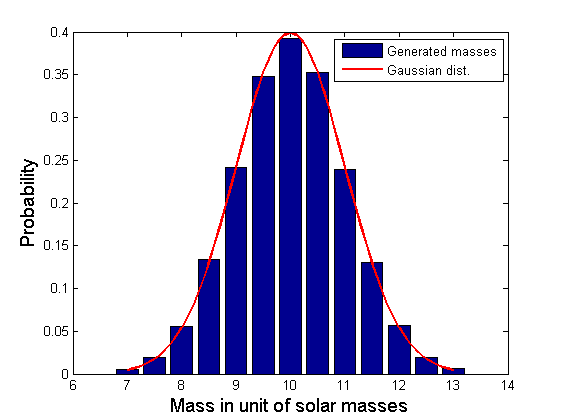
\includegraphics[width=0.7\linewidth]{Figures/random_mass_test.png}
\caption{
Histogram of the mass of 100,000 particles generated by the c++ code introduced \fxnote{where}. 
}
\label{fig:GaussianGeneratedMass}
\end{figure}
\fxnote{eq. include gaussian dist. in fig}

\subsection{Uniformly Distributed Position}
\fxnote{write here, what kind of distribution, we want!}

\begin{lstlisting}
void uniform_pos_generator(mat (&position), int N)
{
double pi=3.14159, c = 2*pi, R = 20;
vec phi(N), r(N), theta(N), x(N), y(N), v(N);

srand(time(NULL));

for (int i=0;i<N;i++){

        x(i) = ((double) rand() / (RAND_MAX)); //random numbers generated in the interval(0,1)
        y(i) = ((double) rand() / (RAND_MAX));
        v(i) = ((double) rand() / (RAND_MAX));
   }
for (int i=0;i<N;i++){
        phi(i)=c*x(i);
        r(i)=R*pow(y(i),1.0/3.0);
        theta(i)=acos(1.0-2.0*v(i));
        position(i,0)=r(i)*sin(theta(i))*cos(phi(i));
        position(i,1)=r(i)*sin(theta(i))*sin(phi(i));
        position(i,2)= r(i)*cos(theta(i));
   }
}
\end{lstlisting}

To test whether the generated positions within the sphere of radius $20$ ly, the density of particles in the cross-sectional area of each $x$-value is determined and plotted as a histogram in \figref{fig:UniformlyGeneratedPos} for $100,000$ particles with position generated by the introduced lines of code.  
The density of particles in the cross-sectional area of each $x$-value is found by dividing the total number of particles with that $x$-value with the cross-sectional area of the sphere in that $x$-value.
The cross-sectional area of the sphere in a specific area is found from a little trigonometry, by first considering that the radius of the circle that makes of the cross-sectional area in a point $x_i$ is given by $r_i = 20sin\theta_i$ ly.  
This yields that the area $A_i$ of the cross-sectional area, in ly, is given as
\begin{align}
	A_i = 400\pi sin^2 \theta_i =  400\pi (1 - cos^2 \theta)
\end{align}
in which the last equal sign stems from $1 = cos^2 \theta + sin^2 \theta$.
But $x_i = 20 cos \theta_i$ ly, giving
\begin{align}
	A_i = \pi (400 - x_i^2)
\end{align}
\begin{figure}[H]
\centering
	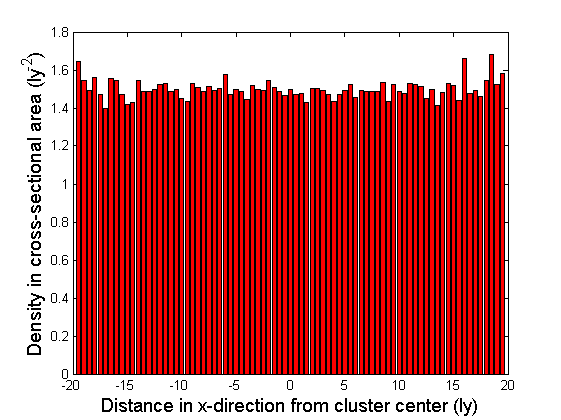
\includegraphics[width=0.7\linewidth]{Figures/random_uniform_position_test.png}
\caption{
Histogram of density of 100,000 particles with position generated by the code introduced in \fxnote{where??} as a function of the $x$-coordinate of the particles. The histogram is made with bins in the interval [$-19.5;19.5$] and a bin-size of $0.5$. The distance $x = \pm 20$ from the cluster center is not considered, since the cross-sectional area in that point is zero.
}
\label{fig:UniformlyGeneratedPos}
\end{figure}
	\chapter{Results and Discussion}
\label{chap:Results}
The starting point is solving the two body system, where Earth- and Sun-like forms the two bodies with masses $1\textrm{M}_{\odot}$ and $3\cdot 10^{-6} \textrm{M}_{\odot}$, respectively, for which $\textrm{M}_{\odot}$ is the solar mass. 
With the help of the Runge-Kutta method and the Velocity-Verlet method introduced in \secref{Newton2body3D}, the problem is solved both with a stationary Sun-like body relative to the frame of reference, and with both Earth and Sun moving relative to the coordinate system, with an initial velocity (0,0,0) and initial position an (1,1,1) for the Sun. 
For earth the initial position is assigned to be (2,1,1) and initial velocity (0,0.017,0). 

For an $N$ body system, the movement of the bodies with the evolution of time is estimated with the Velocity-Verlet method. 
From the result analysis the behaviour of the system is unfold.
\fxnote{ok, is this what we want to do?}

The results from running the codes described in \chapref{chap:method} for computing the blah blah blah ?? can be found in the GitHub folder  \url{https:/??}, together with the MatLab scripts for the plots presented in this chapter. \fxnote{fix these lines}

	\chapter{Conclusion}




	% ¤¤ LITTERATURLISTE: SKAL VÆRE SIDST ¤¤
		\bibliographystyle{ieeetr}
		\bibliography{Bibtex/litteratur}

% ¤¤ BILAG: SKAL VÆRE ALLERSIDST ¤¤
	\appendix

	
\end{document}
